\begin{frame}{A Brief Introduction}
   ``Machine learning, neural networks, and artificial intelligence are increasingly being used in orthopaedics for image processing and analysis tasks. These techniques can be used to {\bf automatically analyze medical images} such as X-rays, MRI scans, and CT scans to {\bf extract important diagnostic information} and help with diagnosis and treatment planning. Machine learning algorithms can be trained to {\bf recognize patterns in the images}, and neural networks can be used to process and interpret the data in a more human-like way. These approaches can be used to {\bf identify abnormalities, measure bone density, and classify different types of tissue}, among other tasks. By automating these processes, doctors and other healthcare professionals can {\bf save time and improve the accuracy of their diagnoses}'' \\
\vspace{5mm}
   \hfill - ChatGPT (emphasis mine)
\end{frame}

\begin{frame}{By the end of this presentation, you should be able to \dots}
   \begin{baseitemize}
      \itemR List some ways that deep learning is being used for image processing in orthopaedics
      \itemR Understand some of the basic neural network architectures, and how those fit into different tasks
      \itemR Have a few tips and tricks up your sleeve for getting started with these networks
      \itemR
   \end{baseitemize}
\end{frame}

\begin{frame}{Three Categories of Deep Learning Applications}
   \renewcommand{\arraystretch}{2}
   \begin{center}
            \begin{tabular}{M{0.3\linewidth}|P{0.6\linewidth}}
               \pause Classification & Identifying objects in images and determining membership in specific classes \pause \\ \hline
               Segmentation & Labeling specific pixels of interest in an image based on desired mask \pause \\ \hline
               Detection & Locating regions in images based on presence of specific object
            \end{tabular}
      \end{center}
\end{frame}

\framecard[colorblue]{{\color{white}\hugetext{EXAMPLES}}}

\begin{frame}
   \centering
      
\includegraphics[width=\linewidth]{images/histology-title.png}
      \vfill
      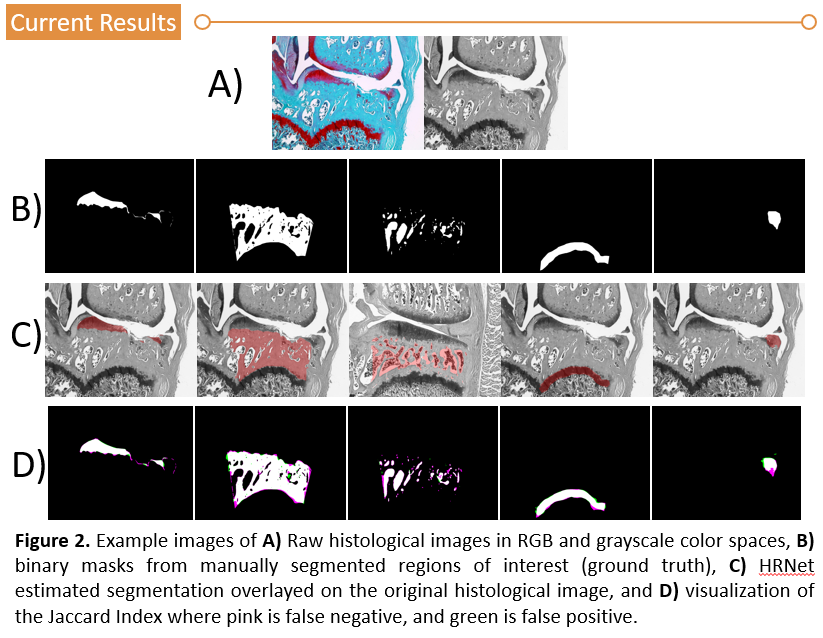
\includegraphics[width=0.65\linewidth]{images/histology-images.png}
\end{frame}

\begin{frame}
   \centering
   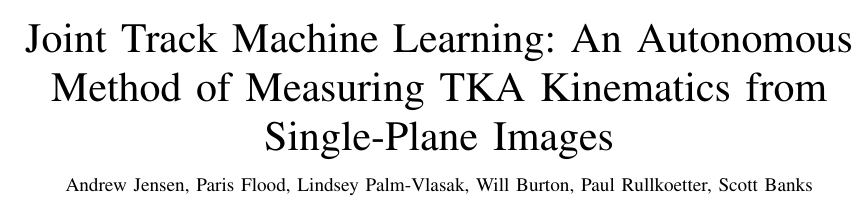
\includegraphics[width=0.78\linewidth]{images/jtml-title.png}
   \vfill
   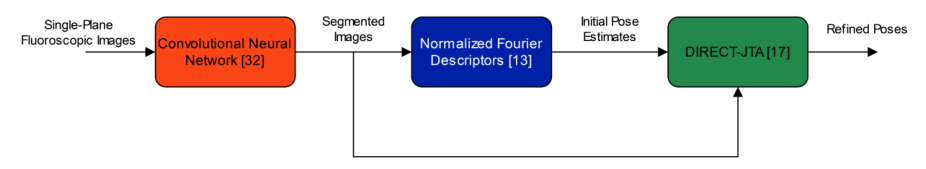
\includegraphics[width=0.75\linewidth]{images/jtml-pipeline.png}
   \vfill
   \begin{columns}
      \begin{column}{0.71\linewidth}
         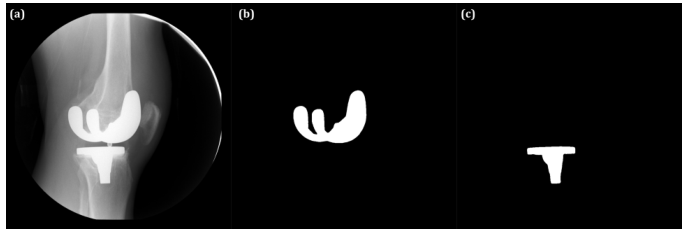
\includegraphics[width=\columnwidth]{images/jtml-nn-image.png}
      \end{column}
      \begin{column}{0.29\linewidth}
         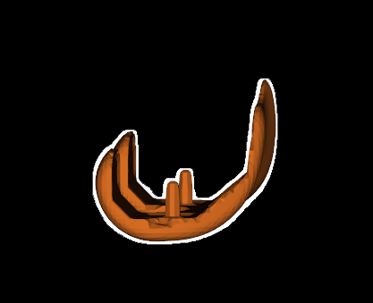
\includegraphics[width=\columnwidth]{images/jtml-registered-implant.png}
      \end{column}
   \end{columns}
\end{frame}

\begin{frame}{Classification of Equine Stifle Pathology}
   \centering
   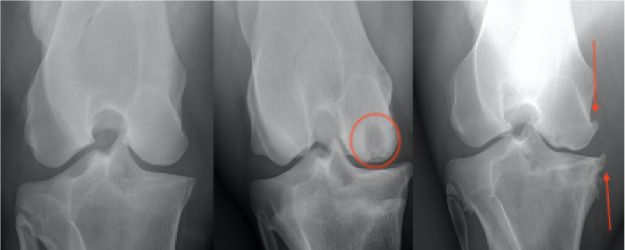
\includegraphics[width=0.85\linewidth]{images/stifle-pathologies.png}
\end{frame}

\begin{frame}
   \centering
   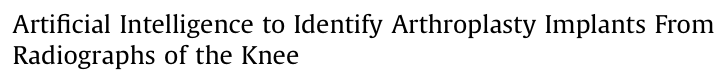
\includegraphics[width=0.7\linewidth]{images/tka-classification-title.png}
   \begin{columns}
      \begin{column}{0.6\linewidth}
         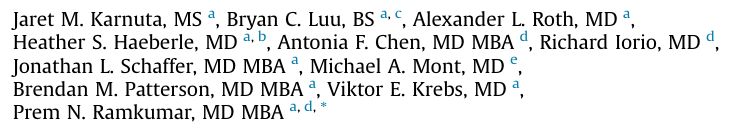
\includegraphics[width=\columnwidth]{images/tka-classification-authors.png}
      \end{column}
      \begin{column}{0.5\linewidth}
         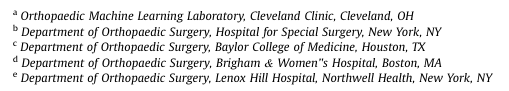
\includegraphics[width=\columnwidth]{images/tka-classification-universities.png}
      \end{column}
   \end{columns}
   \vfill
   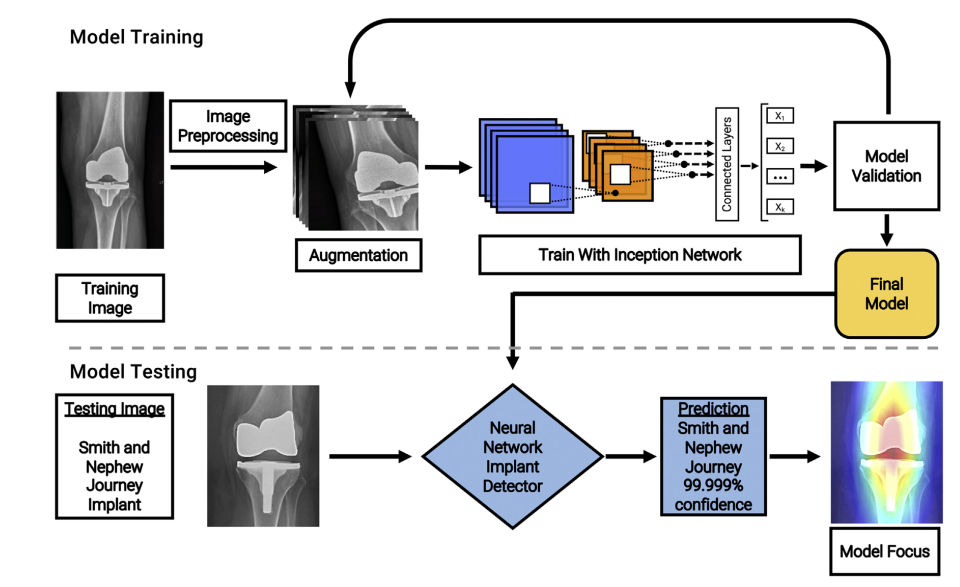
\includegraphics[width=0.65\linewidth]{images/tka-classification.png}
\end{frame}

\begin{frame}
   \centering
   \begin{columns}
      \begin{column}{0.65\linewidth}
         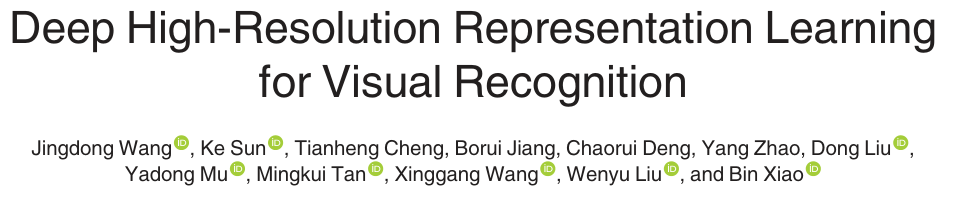
\includegraphics[width=\columnwidth]{images/hrnet-title.png}
      \end{column}
      \begin{column}{0.35\linewidth}
         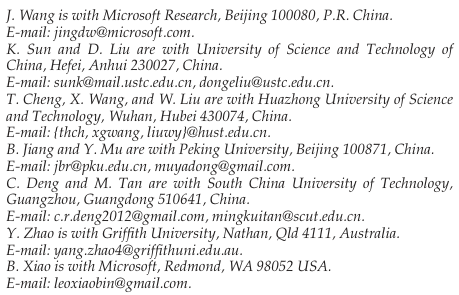
\includegraphics[width=\columnwidth]{images/hrnet-authors.png}
      \end{column}
   \end{columns}
   \vfill
   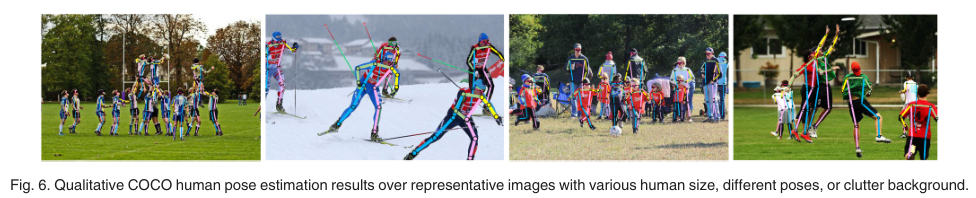
\includegraphics[width=\linewidth]{images/hrnet-human-pose.png}
\end{frame}

\framecard[colorblue]{\color{white}\hugetext{WHAT IS DEEP LEARNING FOR IMAGE PROCESSING?}}

\begin{frame}{A Basic Definition}
   \begin{columns}
      \centering
      \begin{column}{0.4\linewidth}
         \begin{baseitemize}
            \itemR Subset of machine learning using neural networks to imitate the visual system in the brain
            \vspace{0.45in}
            \itemR A set of algorithms that learn programs from data
         \end{baseitemize}
      \end{column}
      \begin{column}{0.6\linewidth}
         \centering
            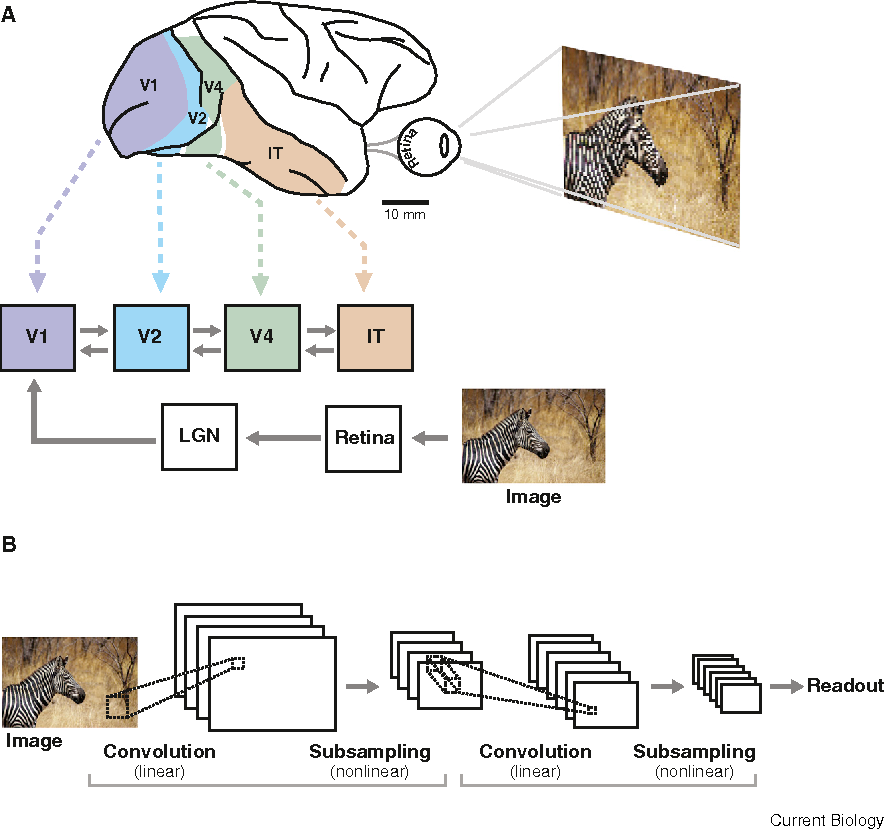
\includegraphics[width=0.8\columnwidth]{images/visual-nn.png}\\
            \tiny{Cox and Dean, Neural Networks and Neuroscience-Inspired Computer Vision, 2014}
      \end{column}
   \end{columns}
\end{frame}


\begin{frame}{The Architecture of a Neural Network}
   \centering
   \renewcommand{\arraystretch}{1.5}
   \begin{tabular}{c|c}
      \Large{Building Block} & \Large{Neural Network} \\ \hline \pause
      {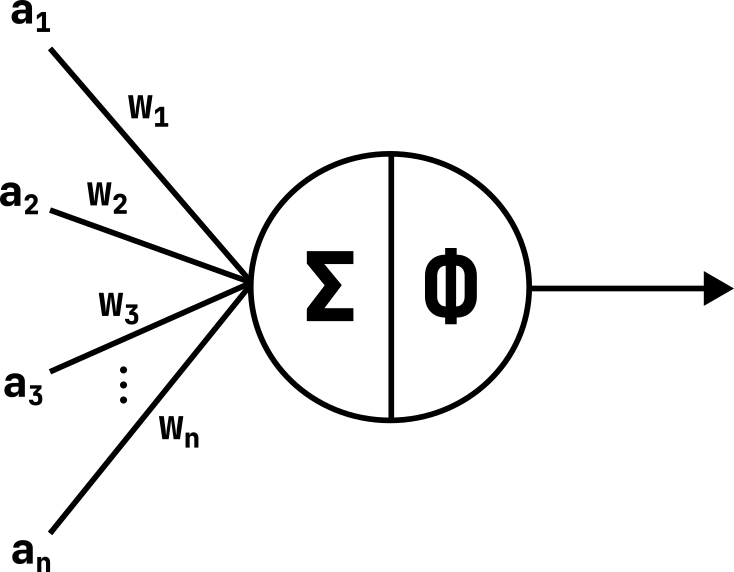
\includegraphics[width=1in, valign=m,margin = 1pt]{images/neuron.png} $\phi(\sum_{i=1}^n a_i w_i)$} & 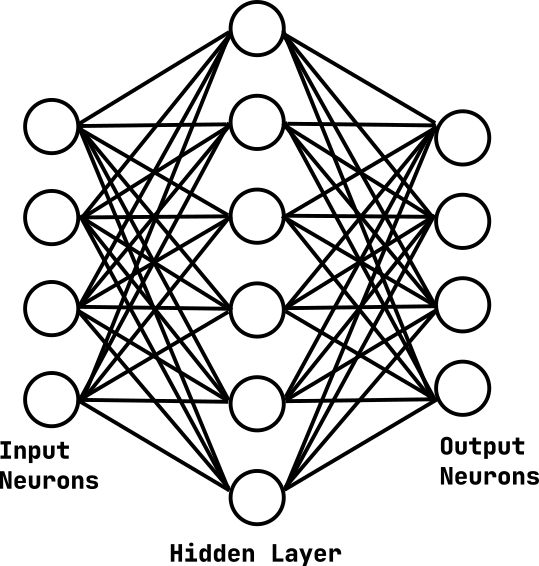
\includegraphics[width=1.25in, valign=m, margin = 1pt]{images/fcn.png} \\ \hline \pause 
      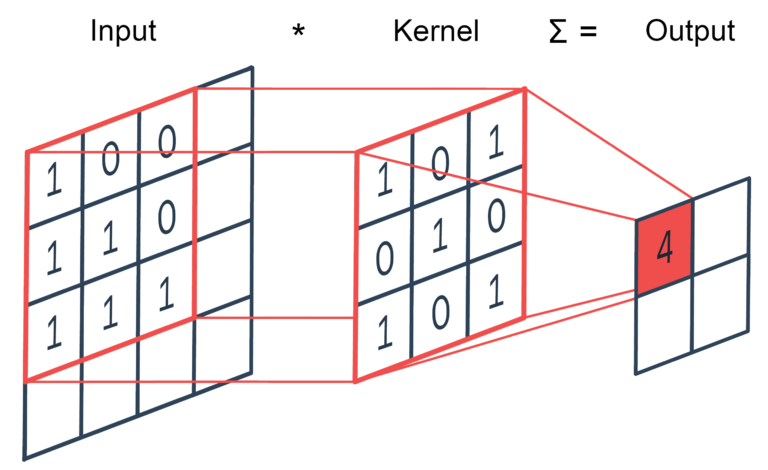
\includegraphics[width = 1.3in, valign=m, margin = 1pt]{images/2d-convolution.png} & 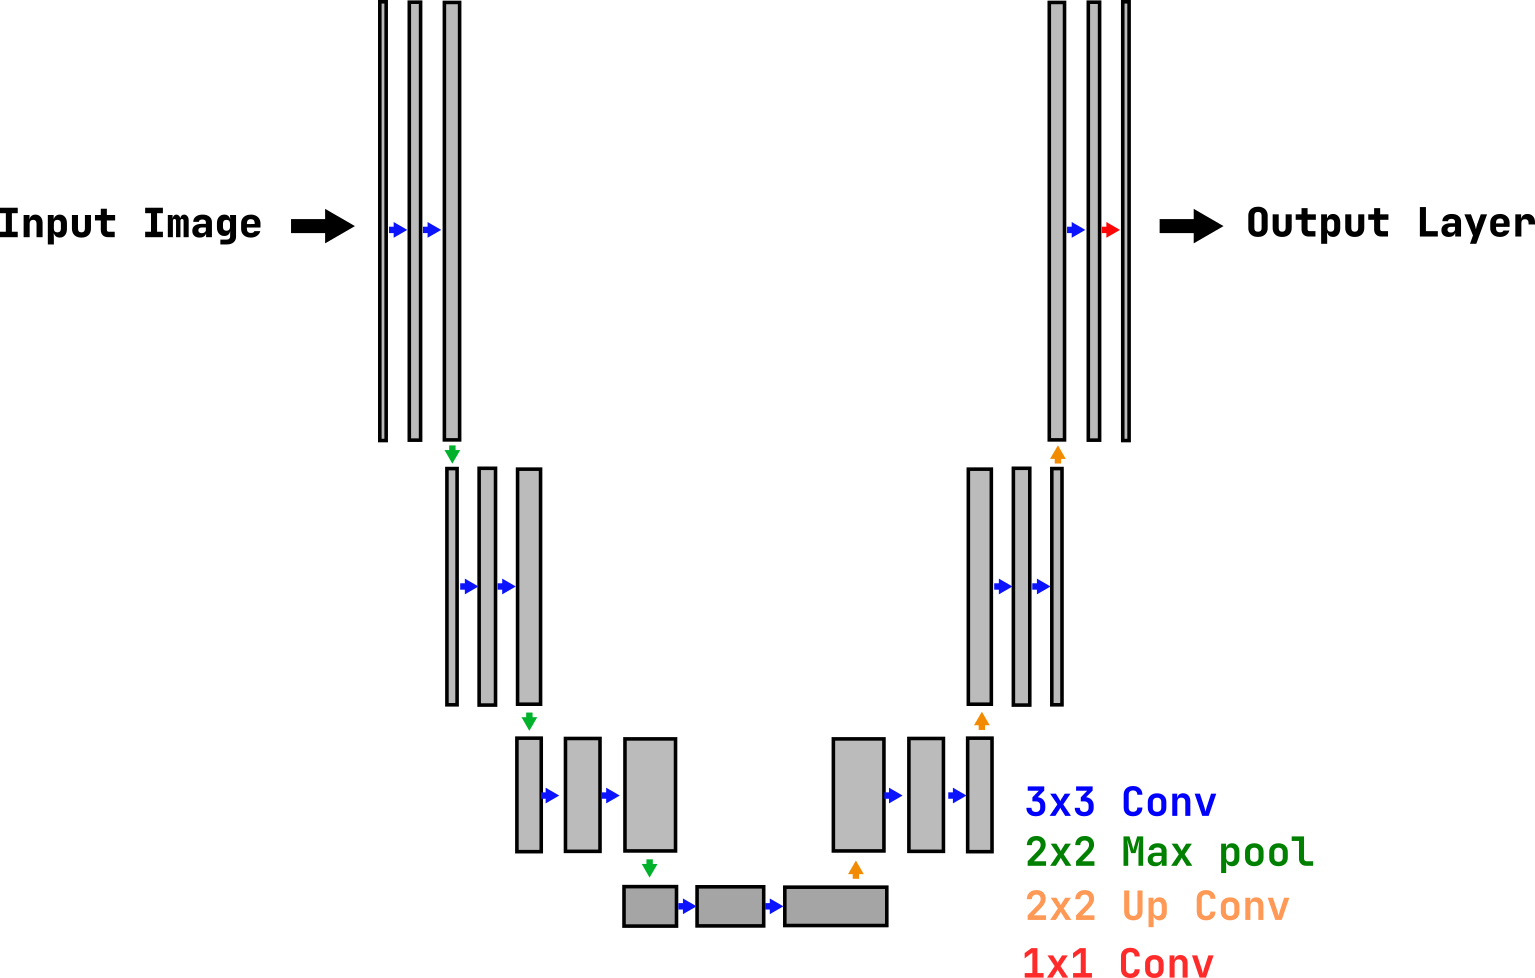
\includegraphics[width=1.85in, valign=m, margin = 1pt]{images/u-net.png}
   \end{tabular}
\end{frame}

\begin{frame}{The Power of Convolutional Neural Networks}
   \centering
   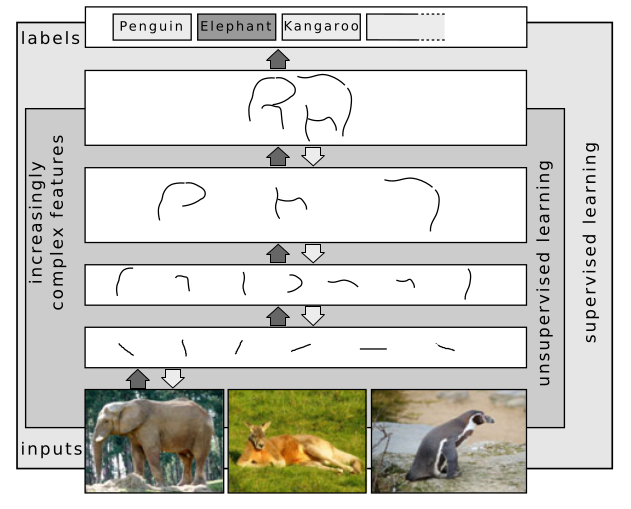
\includegraphics[width=0.6\linewidth]{images/conv-layers.png}\\
   \tiny{Shulz and Behnke, Deep Learning: Layer-Wise Learning of Feature Hierarchies, 2012}
\end{frame}

\framecard[colorblue]{{\color{white}\hugetext{ARCHITECTURE MODIFICATIONS}}}

\begin{frame}{Classification}
   \centering
   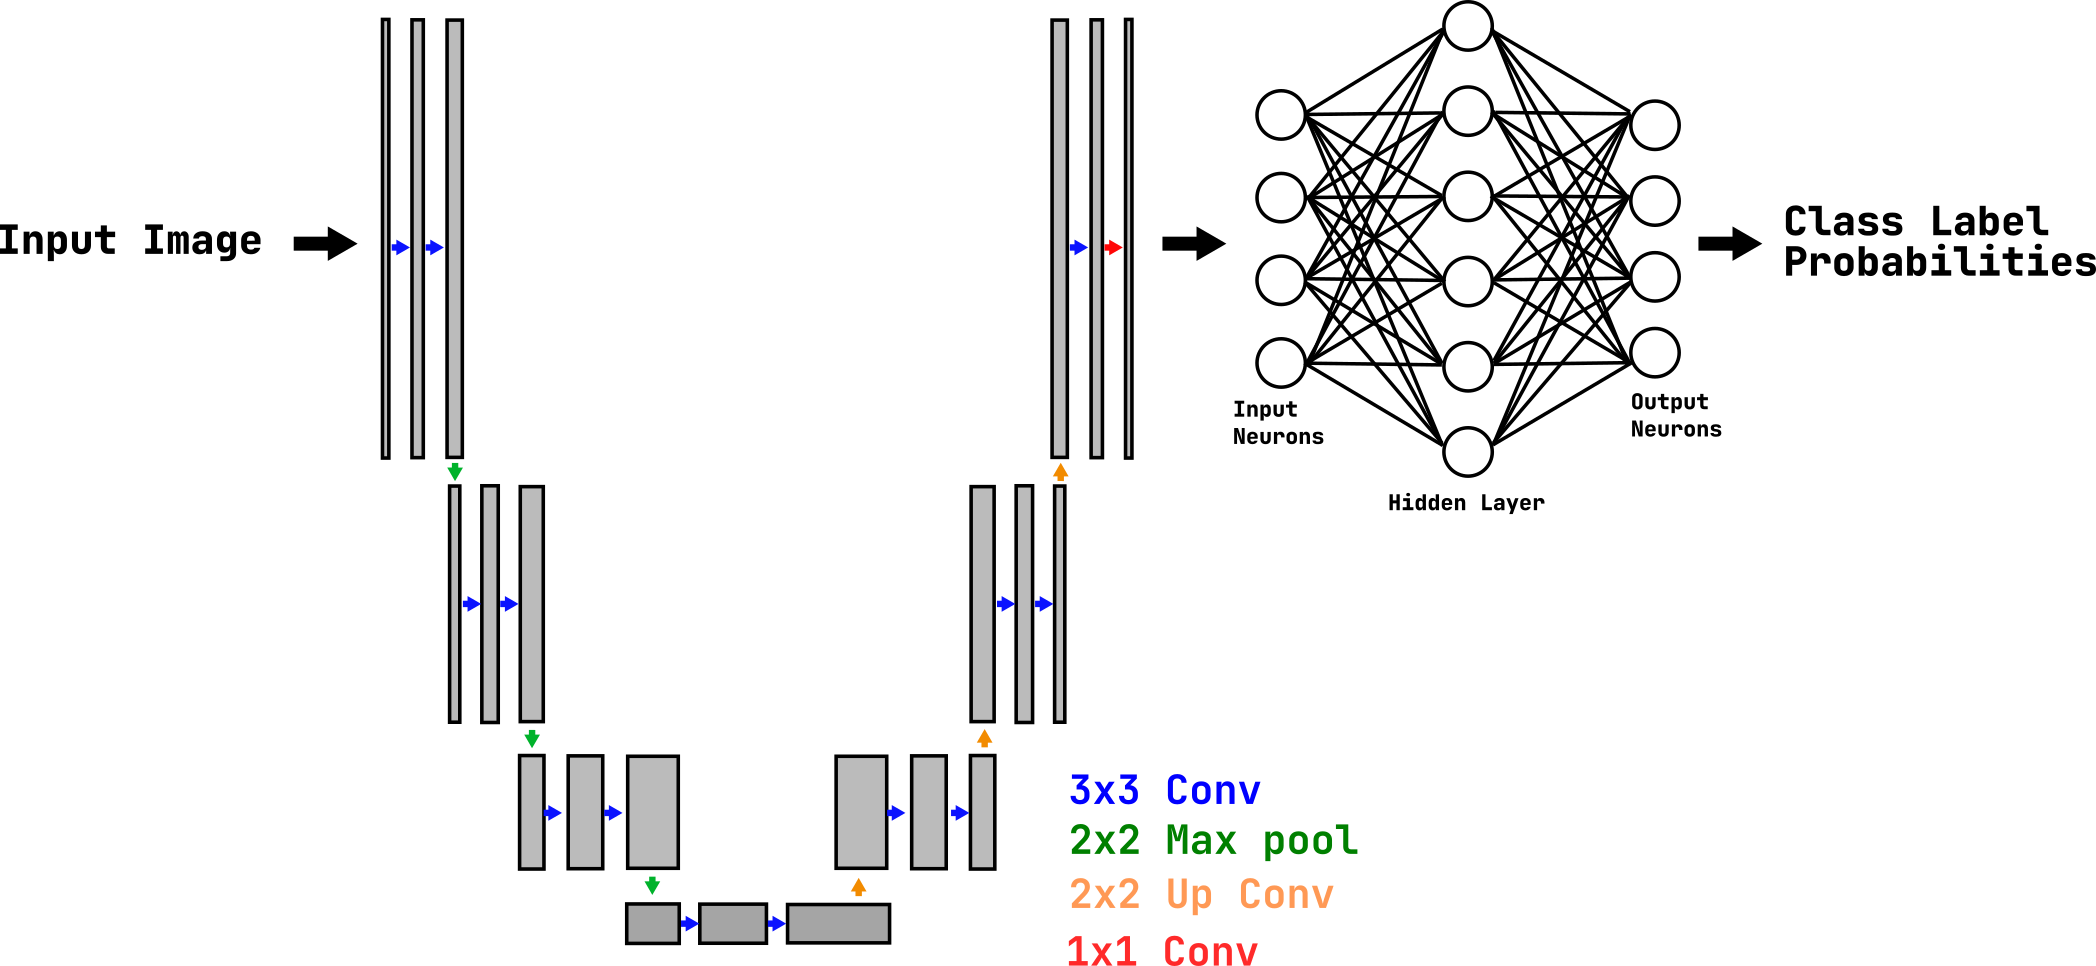
\includegraphics[width=0.8\linewidth]{images/classification.png}
\end{frame}

\begin{frame}{Segmentation}
   \centering
   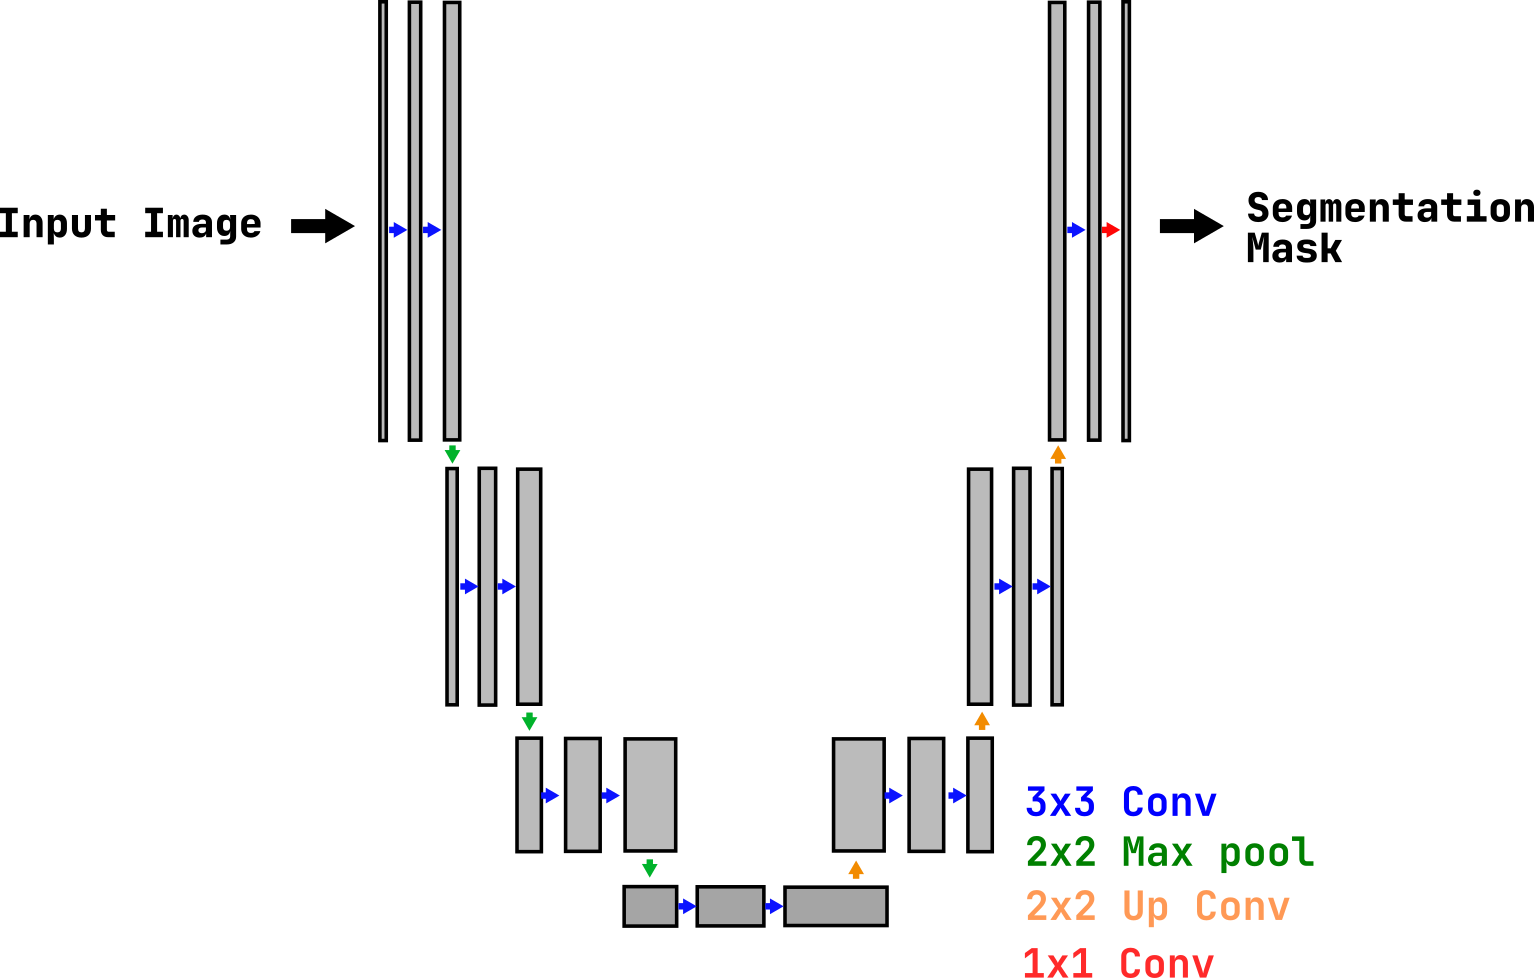
\includegraphics[width=0.8\linewidth]{images/segmentation.png}
\end{frame}
%\begin{frame}{Open Source Fonts}
% \begin{fullpageitemize}
%  \item {\montserratfont This is Montserrat}
%  \item {\notosansfont This is Noto Sans}
%  \item {\latolightfont This is Lato (light)}
%  \item {\inconsolatafont This is inconsolata}
%  \item \textsc{This is Alegreya Sans small caps}
% \end{fullpageitemize}
%\end{frame}


%\begin{frame}{Color Palette}
% \begin{center}
% \crule[colordgray] \crule[colorhgray] \crule[colorblue] \crule[colorgreen] \crule[colororange]
% \end{center}
%\end{frame}

%\framecard[colorgreen]{{\color{white}\hugetext{BIG BOLD TEXT}}}

%\framepic[0.8]{images/skeleton}{
% \begin{textblock}{7}(7,2.5)
%    {\color{colorblue}\hugetext{\textbf{RUN!}}}
% \end{textblock}
%}